\documentclass{article}
\usepackage{amsmath}
\usepackage{amssymb}
\usepackage{fancyhdr}
\usepackage{booktabs}

\usepackage[T1]{fontenc}
\usepackage[utf8]{inputenc}
\usepackage{regexpatch}
\makeatletter
\usepackage{letltxmacro}
\usepackage{aligned-overset}

\usepackage{hyperref}
\usepackage{cleveref}

\usepackage{nowidow}

\usepackage{titling}
\usepackage{braket}
\usepackage{minted}
\usepackage[margin=1in]{geometry}
\usepackage[super]{nth}

\setlength\parindent{0pt}

\title{CMSC32700 Project Report: Verifying Wiesner's quantum money using SQIR}
\author{Adrian E. Lehmann}
\date{Jun 4, 2020}

\begin{document}

\maketitle

\section{Introduction}
At the moment we have many quantum circuit designs, for transmitting and encoding information but none of them have been tried to be verified using SQIR~\cite{SQIR}. 
Hence in this project we will try to verify a simple $n$-qubit quantum key distribution protocol ``Wiesner's quantum money''~\cite{wiesner} which we will examine close in \cref{sec:wiesner}. 
We will then proceed to prove a few interesting properties of the scheme.
The mechanization of said proofs will be described in \cref{sec:proof-impl}.

\section{Background}

\subsection{Coq, QWIRE, SQIR}
To formally verify the algorithm we will be using a quantum formal verification stack based on the coq proof assistant~\cite{coq}.
On top of coq, there are two main libraries that we will be using: QWIRE~\cite{QWIRE} and SQIR~\cite{SQIR}.
QWIRE is a quantum programming language that has been embedded into Coq and SQIR is a fromal verification framework built on top of QWIRE.
While SQIR was originally intended as an intermediate representation for a verified quantum compiler (VOQC~\cite{voqc}), it has been used to prove various algorithms, such as Deutsch-Josza's~\cite{deutsch} or Shor's~\cite{shor} algorithm.


\subsection{Wiesner's qunatum money}\label{sec:wiesner}

Wiesner's quantum money proposed by Stephen Wiesner in 1983~\cite{wiesner}, is a quantum verification scheme that intends to encode an $n$ bit integer. 
Given two parties, Alice and Bob, Alice will encode the n bit integer by choosing a basis such that each bit of the integer will either be encoded to quantum $\ket{1}$ in the basis $\ket{0}, \ket{1}$ or the basis $\ket{-},\ket{+}$.
Physically this corresponds to choice of orthogonal polarization.
Bob will then decode the integer using his basis.
Using the no-cloning property, it follows that when Bob measures to get the classical information, he will certainly get the correct output if his basis is equal.
If his basis does not match, he will have a chance of $\frac{1}{2^{n_{diff}}}$ getting the correct result, where $n_{diff}$ is the number of bits his basis differs from Alice's.
It follows that his chance getting the correct output using a random is $(\frac{3}{4})^n$.

In the context of money, the $n$-bit integer would be a serial number, Alice the central bank, and Bob a malicious \nth{3} party trying to copy money.
While the central bank can validate bills with a given serial numbers, while the \nth{3} party would be unable to decode the bill to get a valid serial number to copy.

\section{Proof Implementation}\label{sec:proof-impl}
We implement a proof to show that Wiesner's quantum money scheme for any $n$ qubits will yield the correct state with probability $1$, if Alice and Bob have the same base, and will only yield the correct output with probability $\frac{1}{2^{n_{diff}}}$, where $n_{diff}$ is the number of bits that are different in Bob's and Alice's base. In the following, we will discuss the steps we took to prove these conjecture. The accompanying code can be found on GitHub\footnote{\url{https://github.com/adrianleh/SQIR/blob/main/examples/Wiesner.v}}.

\subsection{Circuit design}

Our circuit will operate on each qubit independently (i.e. one qubit only influeces the ouput of itself, and the circuit does not require any ancilla), where each qubit will have a Pauli $X$-Gate classically controlled (cc) by a data bit, followed by two Hadamard gates, clasically controlled by Alice's and Bob's basis bits.

Given an input of $\ket{0}$, this will if the data bit is $1$, transform to $\ket{1}$, and then use Alice's basis bit to either stay in the basis $\ket{0},\ket{1}$ basis, or rotate into the $\ket{+},\ket{-}$ basis. 
Bob's basis bit will then control the rotation bob applies to attempt to restore the original basis.

We will now proceed to describing the circuit for $n$ qubits. 
For this we will assume, we have $3$ $n$-sized arrays $data, ab, bb$, containing classical data, basis bits for Alices, and basis bits for Bob respectively.

We designed the circuit inductively, row by row using, such that for our circuit is defined as
$$C(n) = \begin{cases}
I_1&, n=0\\
C(n-1) \otimes R(n)&, n>0
\end{cases}$$,
where $R$ is the function constructing a row
$$R(n) = \begin{cases}X&, data_n = 1\\ I_2&, \text{else}\end{cases} \times \begin{cases}H&, ab_n = 1\\ I_2&, \text{else}\end{cases} \times \begin{cases}H&, bb_n = 1\\ I_2&, \text{else}\end{cases}$$

This is implemented in Coq by the definitions \texttt{circuit'\_qubit\_\_non\_meas} ($\hookrightarrow R(n)$) and \texttt{circuit'}.

An implementation note is that instead of tensoring the constructed unitaries, we chose to append unitaries of dimension $n$, where we solely padded the unitaries to move our operations to the correct qubit.

The coq implementation of this can be seen in \cref{fig:coq-circuit}
\begin{figure}[h]
    \centering
    \begin{minted}[linenos,tabsize=1,breaklines]{coq}
Notation bit_string := (list bool).
Notation combined_bit_string := (list (bool * bool * bool)).    
Definition alice_bit_manip (base : bool) (data : bool) (n i : nat) : base_ucom n :=
  (if data then X i else SKIP);
  (if base then H i else SKIP).
Definition bob_bit_manip (base : bool) (n i : nat) : base_ucom n :=
  if base then H i else SKIP.
Definition circuit'_qubit_i_non_meas (ad ab bb : bool) (n i : nat) : base_ucom n := 
  alice_bit_manip ab ad n i; bob_bit_manip bb n i.

 
Fixpoint circuit'_helper (l : combined_bit_string) (n : nat) (i : nat) : base_ucom n :=
  match l with
    | [] => SKIP
    | ((ad,ab),bb)::l' => circuit'_helper l' n (S i); circuit'_qubit_i_non_meas ad ab bb n i
  end.
    
Definition circuit' (alice_data alice_base bob_base : bit_string) (n : nat) :=
  circuit'_helper (zip (zip alice_data alice_base) bob_base) n 0.
    \end{minted}
    \caption{The QWIRE definition for our circuit}
    \label{fig:coq-circuit}
\end{figure}

We can see the resulting construction in \cref{fig:circuit}

\begin{figure}[h]
    \centering
    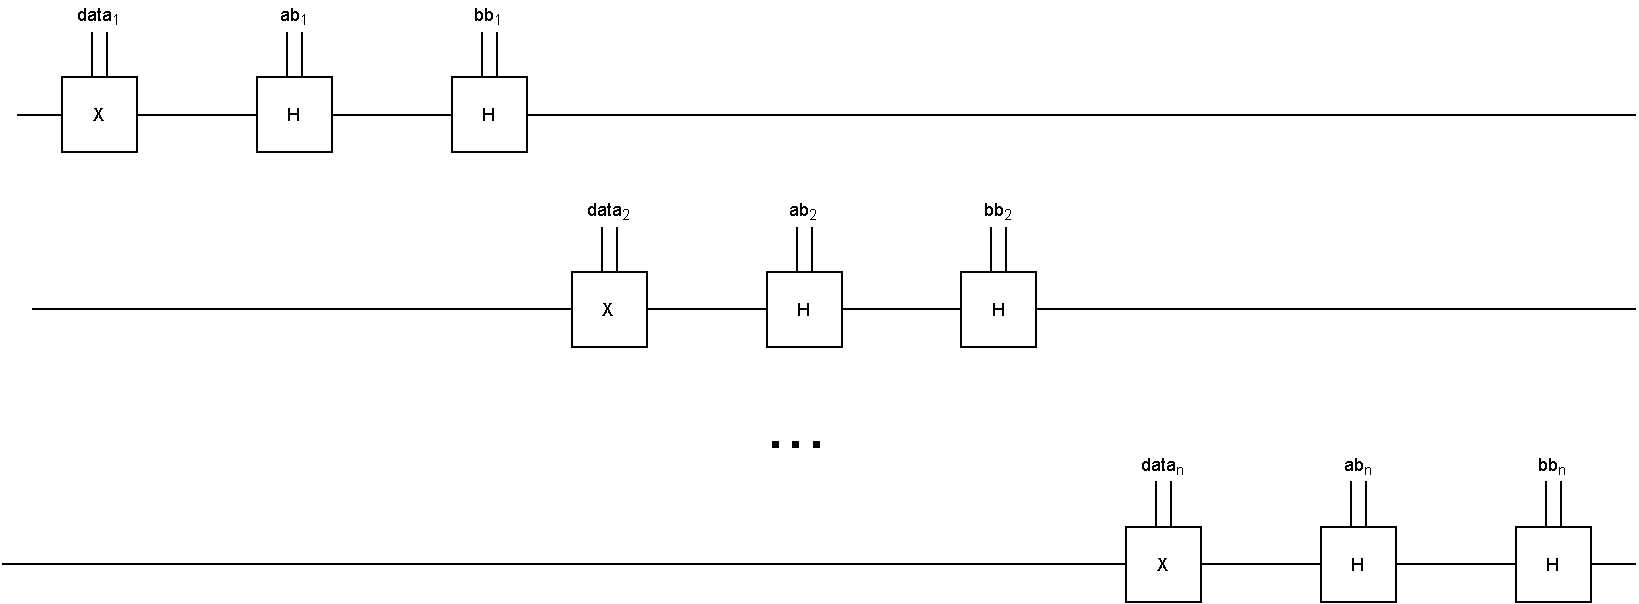
\includegraphics[width=\textwidth]{res/Wiesner.pdf}
    \caption{Wiesner's quantum money for $n$ qubits}
    \label{fig:circuit}
\end{figure}

While some both of these algorithms use $n$ qubits, and use the library feature \texttt{npar} to replicate their circuits, we cannot use this, since each qubit of our circuit depeneds on different classical controls. This fact will complicate our proof and cause us to require the work of \cref{sec:circuit-growth}.

Henceforth we will assume the input to the circuit is initialized to $\ket{\underbrace{0...0}_n}$.

We note that this design is our second iteration, where in the first iteration instead of grouping operations by qubit, we tried grouping them by type (i.e., grouping all the $X$, all of Alice's Hadamard gates, and all of Bob's Hadamard gates) and then concatenating but that turned out to make proof more difficult.

\subsection{Individual qubit correctness}
We prove that for any individual qubit our construction yields 
$\begin{cases} 
\ket{0}&, data=0 \wedge ab=bb\\
\ket{1}&, data=1 \wedge ab=bb\\
\ket{-}&, data=0 \wedge ab \neq bb\\
\ket{+}&, data=1 \wedge ab \neq bb
\end{cases}
$

This proof basically follows directly from the definitions of Pauli $X$ and Hadamard, and the self-inverse property of Hadamard.

In our implementation we proved this through the four lemmata, one for each of the cases listed above.
Though we note that the actual coq lemma prove that the implementation yields gates that trivally transform $\ket{0}$ into said states, instead of proving states directly. 
This proof-design was chosen as operations on unitaries are better supported in SQIR.
\subsection{Inductive circuit correctness}\label{sec:circuit-correct}


\subsection{Inductive circuit growth}\label{sec:circuit-growth}

Likely the most important, yet most challenging lemma to prove was about circuit growth, in the inductive proof that we saw in \cref{sec:circuit-correct} was that state by the coq theorem
\begin{minted}[linenos,tabsize=1,breaklines,escapeinside=||,mathescape=true]{coq}
Theorem circuit'_helper_growth: forall n l, (length l = S n) ->  uc_eval(circuit'_helper l (S (S n)) 1) =  I 2 |$\otimes$| uc_eval (circuit'_helper l (S n) 0).
\end{minted}
which essentially says for any $n>0$ building step $1$ in the inductive construction of a circuit of size $n+1$, the current step is equal to tensoring $I_2$ to the \nth{0} step in building a circuit of size $n$.

Though proving this theorem by itself turned out to be impossible and we resorted to proving a stronger notion where we prove that for a circuit and $n>0$ of size $n+i$, the evaluation of the circuit at step $i+1$ is equal to $I_{i+1}$ tensored with the evaluation of the \nth{0} step of a circuit with size $n$
\begin{minted}[linenos,tabsize=1,breaklines,escapeinside=||,mathescape=true]{coq}
Lemma circuit'_helper_growth_i: forall n l i, (length l = S n) -> uc_eval(circuit'_helper l ((S i) + (S n)) (S i)) =  I (2^(S i)) |$\otimes$| uc_eval (circuit'_helper l (S n) 0).
\end{minted}

The reason we note this property is because this is how we were able to inductively reason about a heterogenous circuit of size $n$ which had been inductively defined.
This theorem is the foundation of any useful reasoning about this circuit.

We note that this circuit growth lemma could likely be generalized to all circuits consisting solely of unitary gates, where each qubit operates independently, and the circuit itself is defined by the same structure of inductive definition. Though this generalization had to be forgone in the interest of time.
\subsection{Individual qubit probability}
\subsection{Inductive circuit probability}

\section{Discussion}

\section{Conclusion}


\bibliographystyle{IEEEtran}
\bibliography{bib}

\end{document}
